\documentclass{article}
\title{CSCI 2200 HW1}
\author{Xinshi,Wang}
\usepackage[letterpaper,textwidth=5.5in,right=0.6in,textheight=9in,left=0.6in,top=0.7in,bottom=0.7in]{geometry}
\usepackage{scrextend}
\usepackage{graphicx}
\usepackage{xcolor}
\usepackage{amssymb}
\usepackage{amsmath}
\usepackage{setspace}
\begin{document}
\noindent
FOCS Quiz 2 \\
Wang Xinshi\\

\noindent (1). D\\
(2). C\\
(3). D\\
(4). C\\
(5). D\\
(6). C\\
(7). D\\
(8). E\\
(9). A\\
(10). C\\
(11). B\\
(12). C\\
(13). D\\
(14). C\\
(15). B\\
(16). C\\
(17). E\\
(18). C\\
(19). C\\
(20). B\\
\newpage

\noindent (1). According to the pigenhole theorem, there has to be at least one more letter than the amount of letters in the alphabet to guarantee two students with the same initials.  Thus choose D.\\\\
(2). $\{\text{Divisible by 2} \cup \text{Divisible by 5}\} = \{\text{Divisible by 2}\}+\text{Divisible by 5}\} = 500+200-100 = 600$. \\\\
(3). Pick 4 from 7.$\binom{7}{4} = \dfrac{7!}{4!3!}$. Choose D.\\\\
(4). $\{CS \cup Bio\} = \{CS\}+\{Bio\}-\{CS \cap Bio\}$, $70 = 50+50-\{CS \cap Bio\}. \{CS \cap Bio\} = 100-70 = 30$.\\\\
(5). The probability for a given probability space is always 1.\\\\
(6). The events that have more heads than tails are HHH,HHT,HTH,THH. The probability of those events occur is $\dfrac{4}{2^3} = \dfrac{4}{2^3} = \dfrac{4}{2^3} = \dfrac{4}{8}$.\\\\
(7). $P(\text{H}|\text{first flip is H})=\dfrac{P(\text{more H} \cap \text{first flip is H})}{P(\text{first flip is H})}$. \\\\
(8). If the first two flips are both H, then it must be the case that there are more heads than tails.\\\\
(9). The probabilities add up to 1. Thus we have $x+2x+3x+4x = 1$. Thus, $x = 0.1$.\\\\
(10). $E[X] = 1 \times 0.1 + 2 \times 0.2 + 3 \times 0.3 + 4 \times 0.4 = 3$.\\\\
(11). We have $P(x = 4)$ and $P(x = 5)$. $\binom{5}{4} \times (\dfrac{1}{3})^4(\dfrac{2}{3})^1 + \binom{5}{5} \times (\dfrac{1}{3})^5 \times 1 = \dfrac{11}{3^5}$\\\\
(12). $E[X] = np = 10 \times \dfrac{1}{2} = 5$.\\\\
(13). The probability of getting a girl is $\dfrac{1}{5}$. $E[X] = \dfrac{1}{p} = \dfrac{1}{\dfrac{1}{5}} = 5$.\\\\
(14). $E[2X_1+X_2+3X_3] = 2E[X_1] + E[X_2] + 3E[X_3] = 2 \times 1 + 2 + 3 \times 3 = 13 $. \\\\
(15). $E[X] = E[X|\text{Men}]P(Men) + E[X|\text{Women}]P(Women) = 5 \times 0.6 + 10 \times 0.4 = 7$\\\\
(16). $P(\text{2 heads})=P(\text{2 heads}|fair)P(fair)+P(\text{2 heads}|\text{two headed})P(\text{two headed}) = \dfrac{\binom{5}{2}}{2^5} \times \dfrac{1}{2} + 0 = \dfrac{\dfrac{5\times4}{2}}{2^5} \times \dfrac{1}{2} = \dfrac{5}{32}$.\\\\
(17). $E[X] = E[X|fair]P(fair)+E[X|two-headed]P(two-headed) = 5 \times \dfrac{1}{2}+10 \times \dfrac{1}{2} = 7.5$.\\\\
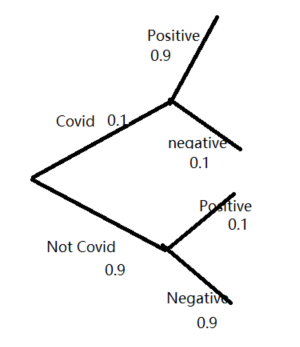
\includegraphics{"C:/Users/Micha/OneDrive - Rensselaer Polytechnic Institute/CSCI 2200/Latex_pictures/atree.png"}\\
(18). If you test positive, it could be false positve or true positive. Thus $P(Covid|Positive) = \dfrac{P(Covid \cap Positive)}{P(Positive)} = \dfrac{0.1 \times 0.9}{P(Positive \cap no-covid)+P(Positive \cap Covid)} = \dfrac{0.1 \times 0.9}{0.9 \times 0.1 + 0.1 \times 0.9} = \dfrac{1}{2} = 50\% $.\\\\
(19). $E[\#Positive] = E[\#Positive \cap FalsePositive]P(FalsePositive)+E[\#Positive \cap TruePositive]P(TruePositive) = 100 \times 0.1 \times 0.9 + 100 \times 0.1 \times 0.9 = 18$.\\\\
(20). Assume there are two colors A and B. Then the sample space has AA, BB, AB, AA. $E[X] = E[X|AA]P(AA)+E[X|BB]P(BB)+E[X|AB]P(AB)+E[X|BA]P(BA) = (1+\dfrac{1}{1-\dfrac{1}{4}}) \times \dfrac{1}{4} + (1+\dfrac{1}{1-\dfrac{1}{4}}) \times \dfrac{1}{4} + 1 \times \dfrac{1}{4} + \dfrac{1}{4} \times 1 = (1+\dfrac{4}{3}) \times \dfrac{1}{4} \times 2 + \dfrac{1}{2} = \dfrac{7}{3} \dfrac{1}{2} + \dfrac{1}{2} = \dfrac{10}{6} = \dfrac{5}{3}$.
\end{document} 